\subsubsection*{Le choix d'architecture : un cerveau et un exécutant}

Je cherche un système qui lise les capteurs, décide, commande les pompes et se laisse surveiller à distance. Le Raspberry Pi 3 B est un vrai petit ordinateur : il garde l'historique, fait tourner un serveur web et peut être programmé en Python. Mais il n'a pas d'entrées analogiques et il peut se bloquer. L'Arduino Uno R3 n'a presque aucune mémoire, mais il lit les capteurs de façon fiable et fait ce qu'on lui demande, sans jamais s'arrêter. Je répartis donc les rôles ainsi :

\textbf{Le Raspberry Pi est le cerveau.} Il tourne sous Python (programme \texttt{cerveau.py}), garde les mesures dans une base de données, décide quand doser et quand faire circuler l'eau, et sert le dashboard.

\textbf{L'Arduino est l'exécutant et le garde-fou.} Il lit les capteurs en valeurs brutes, commande les pompes sur ordre du Pi, et applique seul les sécurités. Toute la logique est sur le Pi, toute la protection est sur l'Arduino : si le Pi plante, la tour ne peut pas se noyer ni se vider.

Les deux cartes communiquent par le câble USB, à \qty{115200}{bauds}, par des lignes de texte. Le Pi envoie des ordres courts et l'Arduino répond.

\begin{table}[H]
\centering
\small
\begin{tabularx}{\textwidth}{|c|Y|Y|}
\hline
\textbf{Ordre du Pi} & \textbf{Ce qu'il demande} & \textbf{Réponse de l'Arduino} \\
\hline
\texttt{P} & Es-tu là ? & \texttt{OK P} \\
\hline
\texttt{L} & Lis tous les capteurs & une ligne \texttt{M} avec pH, EC, niveau, température de l'eau et de l'air, humidité, lumière, inclinaison \\
\hline
\texttt{D <c> <ms>} & Fais tourner la pompe $c$ pendant $ms$ millisecondes (0 : circulation, 1 : engrais A, 2 : engrais B, 3 : pH$-$) & \texttt{OK D ...} ou \texttt{ERR ...} \\
\hline
\texttt{S} & Arrête toutes les pompes & \texttt{OK S} \\
\hline
\texttt{E} & Donne ton état & état des pompes, du mode secours, de la chute, du niveau \\
\hline
\texttt{N}, \texttt{Z}, \texttt{R} & Règle le seuil de niveau, mémorise la tour droite, réarme après une chute & \texttt{OK ...} \\
\hline
\end{tabularx}
\caption{Les ordres échangés entre le Raspberry Pi et l'Arduino.}
\end{table}

\subsubsection*{Les sécurités de l'Arduino}

Chaque durée de pompe est limitée : \qty{30}{s} au maximum pour une doseuse (\qty{30000}{ms}) et \qty{1000}{s} pour la circulation. Un ordre trop long reçoit la réponse \texttt{ERR duree}. L'Arduino applique ensuite quatre protections.

\textbf{Le niveau bas.} Si le niveau d'eau passe sous le seuil réglé, la circulation est coupée (une pompe qui tourne à sec s'abîme), mais les doseuses restent permises. Elle reprend quand le niveau remonte de plus de \qty{50}{mV} au-dessus du seuil (hystérésis\ix{31}, pour éviter de couper et reprendre sans cesse).

\textbf{La chute.} Si la tour penche de plus de \ang{35} pendant plus d'une seconde (calcul de la partie 7), toutes les pompes s'arrêtent et refusent tout ordre, jusqu'à ce que la tour soit redressée et réarmée.

\textbf{Le chien de garde.} Si le programme de l'Arduino se bloque pendant plus de \qty{8}{s}, il redémarre seul, et toutes les pompes repartent à l'arrêt.

\textbf{Le mode secours.} Si le Pi n'envoie plus rien pendant 5 minutes, l'Arduino passe en mode secours : la circulation tourne \qty{15}{min} puis s'arrête \qty{15}{min}, sans aucun dosage. Dès qu'un ordre arrive, le mode secours s'arrête. Ainsi, une panne du Pi ne tue pas les plantes : l'eau continue de circuler.

\subsubsection*{Le pilotage : planning, cibles et dosage}

Le Pi suit un planning de circulation : de 6 h à 18 h, \qty{15}{min} de marche puis \qty{15}{min} d'arrêt ; la nuit, \qty{15}{min} à 21 h, 0 h et 3 h. L'Arduino limite une commande à environ \qty{1000}{s} : pour une marche de \qty{15}{min}, le Pi envoie un ordre de \qty{90}{s} qu'il renouvelle toutes les minutes environ (un « bail »). Si le Pi se tait, la pompe s'arrête d'elle-même au bout de \qty{90}{s}.

Les cibles viennent de la recherche documentaire sur les besoins des plantes. Pour la laitue en croissance des feuilles, le pH visé est de 5,6 à 6,0 et l'EC de \qtyrange{1,2}{1,6}{mS/cm} (\qtyrange{1200}{1600}{\micro S/cm}) ; le dosage vise le milieu de la plage, soit environ \qty{1,4}{mS/cm}. L'alarme de température de l'eau se déclenche au-dessus de \qty{28}{\celsius}. Le dashboard contient le tableau des légumes (laitue, tomate cerise, poivron) avec leurs plages par stade de croissance.

\naturecalc{théorie (hypothèses à mesurer : sensibilité de l'EC et débit des doseuses)}
\begin{demonstration}[volume d'engrais pour remonter l'EC]
\resultat{V_A = \dfrac{(EC_{cible} - EC_{mes})\; V_{bac}}{s}}
Je note $EC_{mes}$ l'EC mesurée, en mS/cm, $EC_{cible}$ la cible, en mS/cm, $V_{bac}$ le volume du bac, en litres (\qty{152}{L}), $V_A$ le volume de solution mère A à ajouter, en mL (le même volume de B est ajouté), et $s$ l'augmentation d'EC provoquée par \qty{1}{mL} de A et \qty{1}{mL} de B par litre de bac, en (mS/cm)/(mL/L). Je prends $s = \qty{0,56}{(mS/cm)/(mL/L)}$ (hypothèse à mesurer). En solution diluée, l'EC est proportionnelle à la quantité de sels. Elle augmente donc proportionnellement à la dose $d$ (en mL par litre de bac) :
\begin{align*}
\Delta EC &= s\,d
\end{align*}
La dose est le volume ajouté divisé par le volume du bac, $d = V_A/V_{bac}$. En remplaçant et en isolant $V_A$ :
\begin{align*}
\Delta EC &= s\,\frac{V_A}{V_{bac}}\\
V_A &= \frac{\Delta EC\; V_{bac}}{s}
\end{align*}
Avec $\Delta EC = EC_{cible} - EC_{mes}$. Application : EC mesurée \qty{1,20}{mS/cm}, cible \qty{1,40}{mS/cm} :
\begin{align*}
V_A &= \frac{(\qty{1,40}{mS/cm} - \qty{1,20}{mS/cm}) \times \qty{152}{L}}{\qty{0,56}{(mS/cm)/(mL/L)}}\\
V_A &= \frac{\qty{30,4}{mS/cm\cdot L}}{\qty{0,56}{(mS/cm)/(mL/L)}}\\
V_A &\approx \qty{54,3}{mL}
\end{align*}
La durée de marche d'une pompe de débit $Q$ est le volume divisé par le débit, $t = V/Q$. Avec $Q = \qty{80}{mL/min}$ (hypothèse à mesurer, mesure M5) :
\begin{align*}
t &= \frac{\qty{54,3}{mL}}{\qty{80}{mL/min}} \approx \qty{0,679}{min} \approx \qty{40,7}{s}
\end{align*}
Cette durée dépasse la limite de \qty{30}{s} : le Pi découpe la dose en deux ordres d'environ \qty{20,4}{s}, espacés pour laisser l'eau se mélanger, et il mesure de nouveau l'EC avant de continuer.
\end{demonstration}

\subsubsection*{Le serveur et le dashboard}

Le Pi héberge un serveur web écrit en Python avec Flask (programme \texttt{server.py}, port 5000), protégé par un identifiant et un mot de passe. Il enregistre toutes les mesures dans une base SQLite, avec l'heure en temps universel, et répond à des adresses web simples : les dernières mesures, l'historique, le journal des actions et un export des données au format CSV. La page du dashboard (\texttt{hydrotour.html}) se met à jour toutes les 10 secondes. Pour y accéder depuis l'extérieur sans toucher à la box Internet, je passe par Tailscale\ix{20} ; Raspberry Pi Connect permet en plus de prendre la main sur le Pi. Les captures ci-dessous viennent du dashboard branché sur un Arduino simulé.

\begin{figure}[H]
\centering
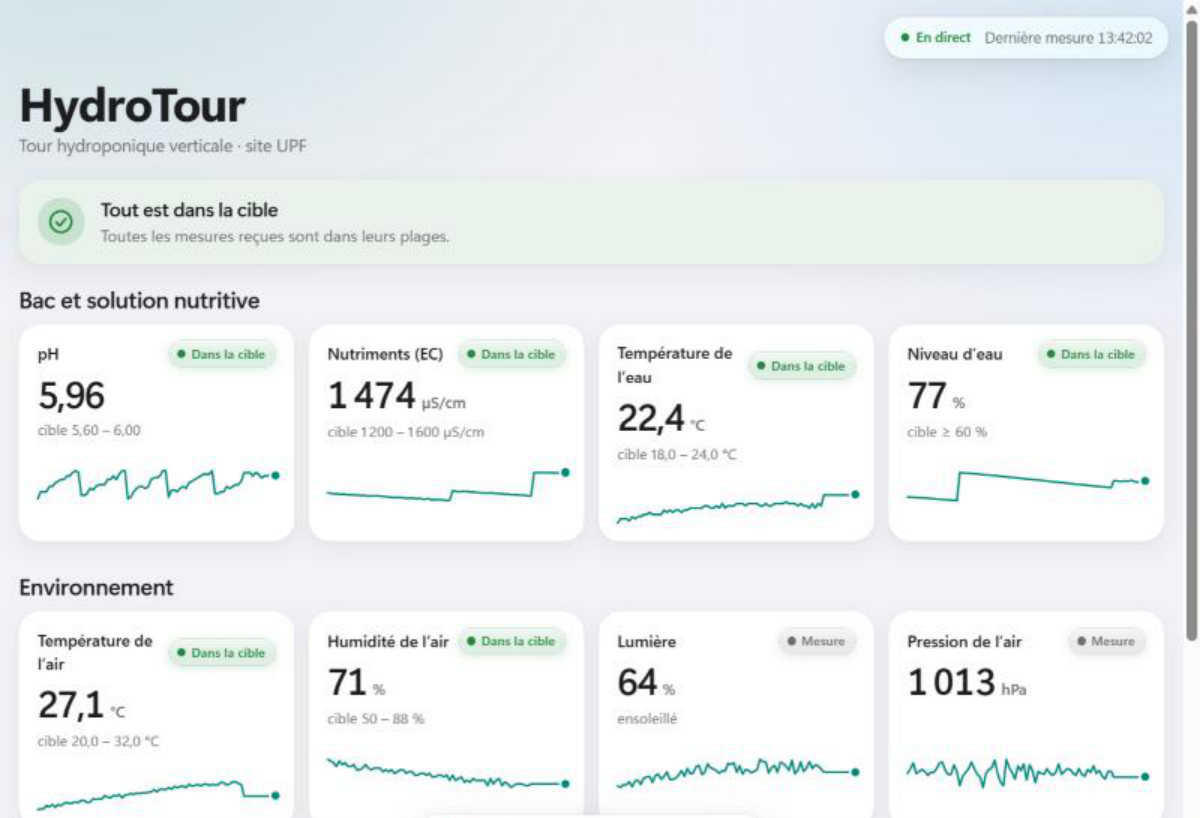
\includegraphics[width=0.82\textwidth]{img/dash_mesures.png}
\caption{Onglet Mesures : chaque tuile indique la valeur, la cible du légume et la courbe des dernières heures ; le bandeau du haut résume l'état.}
\end{figure}

\begin{figure}[H]
\centering
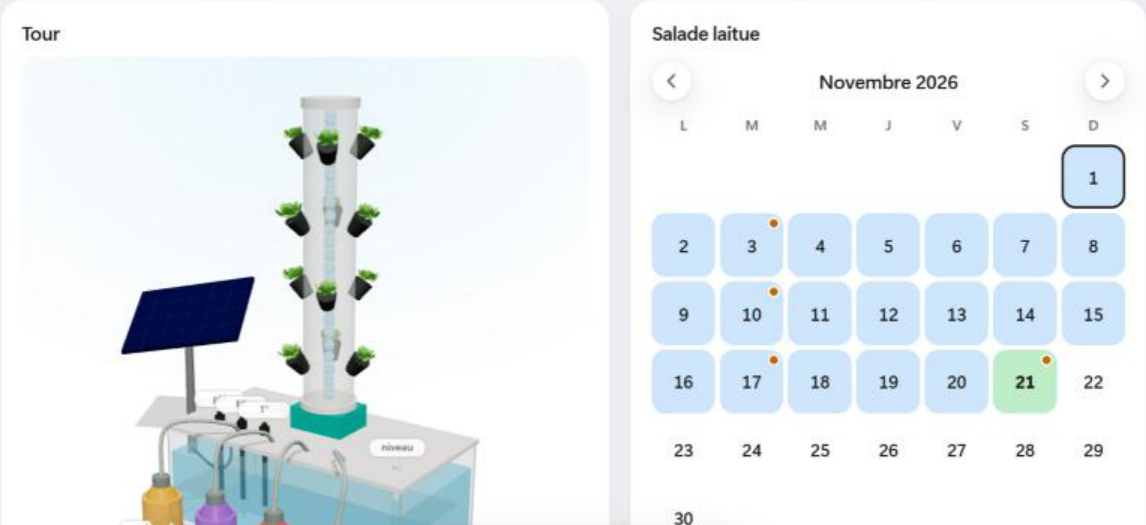
\includegraphics[width=0.82\textwidth]{img/dash_tour.png}
\caption{Onglet Installation : la tour en 3D suit le stade de la plante et le calendrier rappelle les contrôles.}
\end{figure}

\begin{figure}[H]
\centering
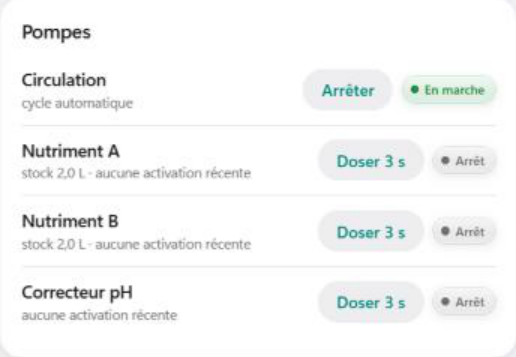
\includegraphics[width=0.55\textwidth]{img/dash_pompes.png}
\caption{Carte des pompes : état de chacune, dose manuelle de \qty{3}{s} et stock d'engrais restant.}
\end{figure}

\begin{figure}[H]
\centering
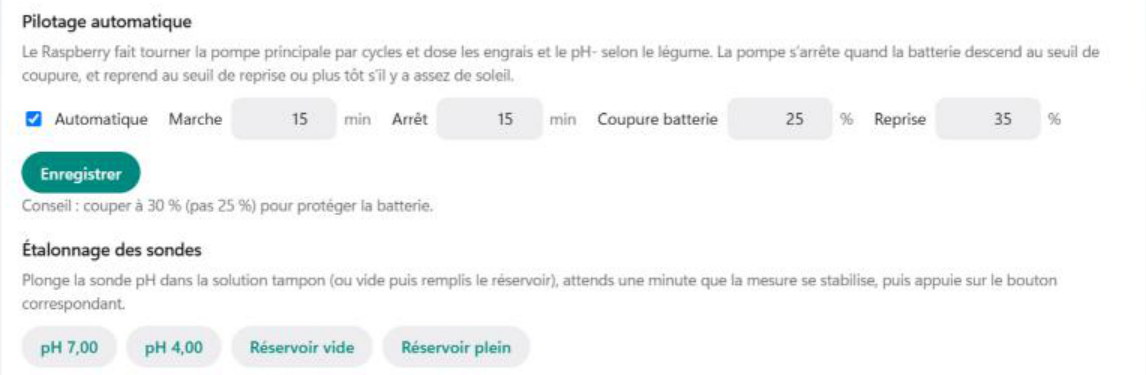
\includegraphics[width=0.9\textwidth]{img/dash_param.png}
\caption{Réglages du pilotage automatique et étalonnage des sondes (pH 7, pH 4, réservoir vide, réservoir plein).}
\end{figure}

Pour se rendre compte du fonctionnement réel du site, j'ai publié une copie de démonstration du dashboard, identique à l'interface réelle mais alimentée par des mesures fictives et figées : \href{https://claude.ai/artifact/G8rZH2kN7ZYfnY5RFY4Tiu}{\textbf{ouvrir le dashboard de démonstration}} (adresse complète : \url{https://claude.ai/artifact/G8rZH2kN7ZYfnY5RFY4Tiu}). La page s'ouvre sur l'écran de connexion. L'identifiant est \texttt{demo} et le mot de passe est \texttt{hydrotour-demo}. Il faut aussi recopier les cinq caractères du captcha affiché (le bouton « Autre image » en génère un nouveau). Les quatre onglets se parcourent comme sur la tour. Les ordres envoyés aux pompes n'agissent sur aucun matériel, et l'export du journal ne fonctionne pas dans cette version.

Un appui manuel sur la circulation met l'automatique en pause : sans cela, le Pi rallumerait la pompe dix secondes plus tard. Le serveur refuse les réglages absurdes, par exemple une reprise trop proche du seuil de coupure de la batterie.

\subsubsection*{Ce qui est fait et ce qui ne l'est pas}

\textbf{Vérifié sur le vrai matériel :} la sonde de pH étalonnée dans des solutions de référence, la chaîne de la sonde jusqu'au téléphone, le dashboard avec un Arduino simulé. \textbf{Compilé mais pas essayé sur la carte :} le programme de l'Arduino (flash \qty{23216}{octets} sur \qty{32256}{octets}, soit 72\,\% ; mémoire vive \qty{681}{octets} sur \qty{2048}{octets}, soit 33\,\%). \textbf{Compilé mais pas encore relu en entier :} \texttt{cerveau.py} (environ 1400 lignes). \textbf{Reste à faire :} un faux Arduino pour tester sans matériel, la relecture de \texttt{cerveau.py}, le script d'étalonnage, le fichier de configuration et le démarrage automatique du programme au branchement.

\begin{aretenir}
Le Raspberry Pi décide, l'Arduino exécute et protège : niveau bas, chute au-delà de \ang{35}, chien de garde de \qty{8}{s} et mode secours de la circulation après 5 minutes de silence. Une dose d'engrais se calcule par $V_A = \Delta EC\,V_{bac}/s$ (\qty{54}{mL} pour passer de \qty{1,20}{mS/cm} à \qty{1,40}{mS/cm}, hypothèses à mesurer). Le dashboard permet de tout surveiller et régler depuis un téléphone. Le programme de l'Arduino n'a pas encore tourné sur la carte.
\end{aretenir}

